
\section{Introduction to Qt}

Qt Creator is a complete IDE for creating applications with Qt Quick and the Qt application framework.
Qt  is  designed  for  developing  applications  and  user  interfaces  once  and  deploying  them  across  several
desktop and mobile operating systems.
One  of  the  major  advantages  of  Qt  Creator  is  that  it  allows  a  team  of  developers  to  share  a  project
across  different  development  platforms  (Microsoft  Windows,  Mac  OS  X,  and  Linux)  with  a  common
tool  for  development and debugging. In addition, UI  designers can join the team by using Qt Quick tools
for creating fluid user interfaces in close cooperation with the developers.
The  main  goal  for  Qt  Creator  is  meeting  the  development  needs  of  Qt  Quick  developers  who  are
looking  for  simplicity, usability, productivity, extendibility and openness,  while aiming  to lower the barrier
of  entry  for  newcomers  to  Qt  Quick  and  Qt.  The  key  features  of  Qt  Creator  allow  UI  designers  and
developers to accomplish the following tasks:
\begin{itemize}
\item Get  started  with  Qt  Quick  application  development  quickly  and  easily  with  examples,  tutorials,
and project wizards.
\item Design  application  user  interface  with  the  integrated  editor,  Qt  Quick  Designer,  or  use graphics
software to design the user interface and use scripts to export the design to Qt Quick Designer.
\item Develop  applications   with  the   advanced  code  editor  that  provides  new  powerful  features  for
copleting code snippets, refactoring code, and viewing the element hierarchy of QML files.
\item Build  and  deploy  Qt  Quick  applications  that  target  multiple  desktop and mobile platforms, such
as Microsoft Windows, Mac OS X, Linux, Symbian, MeeGo, and Maemo.
\item Debug  JavaScript  functions  and  execute  JavaScript  expressions  in  the  current  context,   and
inspect QML at runtime to explore the object structure, debug animations, and inspect colors.
\item Profile  your  Qt  Quick  applications  with  the  QML  Profiler.  You can inspect binding evaluations,
signal  handling,  and  painting  operations  when  running  QML  code.  This  is  useful  for  identifying
potential bottlenecks, especially in the evaluation of bindings.
\item Deploy  applications  to  mobile  devices  and  create  application  installation  packages  for  Symbian
and Maemo devices that can be published in the Ovi Store and other channels.
\item Easily access information with the integrated context­sensitive Qt Help system.
\item It has differents modes such as Welcome, edit debug, design,analyze and help
\end{itemize}


\section{Working with Qt Creator}

Qt  Creator  meets  its  design  goals  of  simplicity,  ease­of­use,  and  productivity  by  relying  on the concept
of  modes.  These  adapt  the   user  interface  to  the  different  application  development  tasks  at  hand.  When
developers  start  Qt  Creator, it opens to  the Welcome mode, where they  can open tutorials and example
projects or start the project wizard to create their own projects.

\begin{figure}[h]
\begin{center}
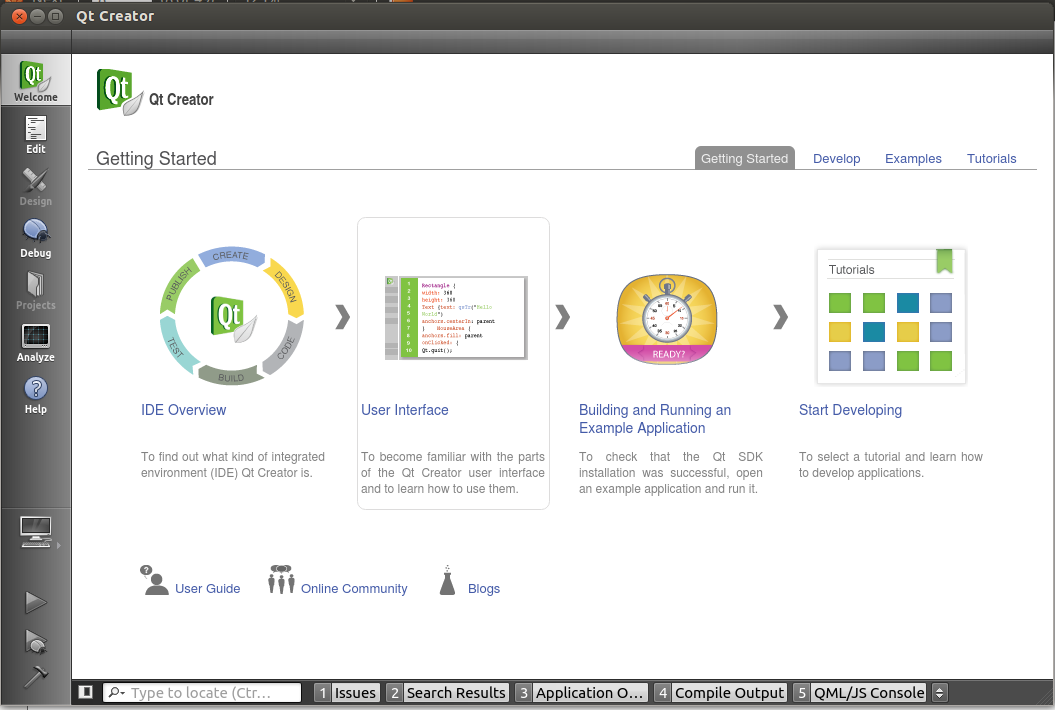
\includegraphics[scale=0.4]{images/Qt.png}
\caption{Welcome screen of Qt Creator}
\end{center}
\end{figure}

Each  mode  has  its  own  view  that  shows  only  the  information  required  for  performing  a  given  task,   and
provides  only  the  most  relevant  features  and  functions  related  to  it.  As  a  result,  the  majority  of  the  Qt
Creator window area is always dedicated to actual application development tasks.
Users  can  employ  the  mode  selector  to  switch  to  a  Qt  Creator  mode.  The  following  image  displays an
example application in Edit mode and Design mode.

\begin{figure}[h]
\begin{center}

\includegraphics[scale=0.8]{images/welcome.png}
\end{center}
\caption{Welcome mode in Qt}
\end{figure}
\begin{figure}[!h]
\begin{center}

\includegraphics[scale=0.8]{images/edit.png}
\caption{Edit mode in Qt}
\end{center}
\end{figure}

\newpage



\subsection{Creating Projects}

To  be  able  to  build  and  run  applications,  Qt  Creator  needs  the  same  information  as  a  compiler  would
need.  This  information  is  specified  in  the  project  build  and  run  settings.  Setting  up  a  new  project  in  Qt
Creator  is  aided  by  a  wizard  that  guides  the  user  step­by­step  through  the  project  creation  process. 
\begin{figure}[htb]
\begin{center}
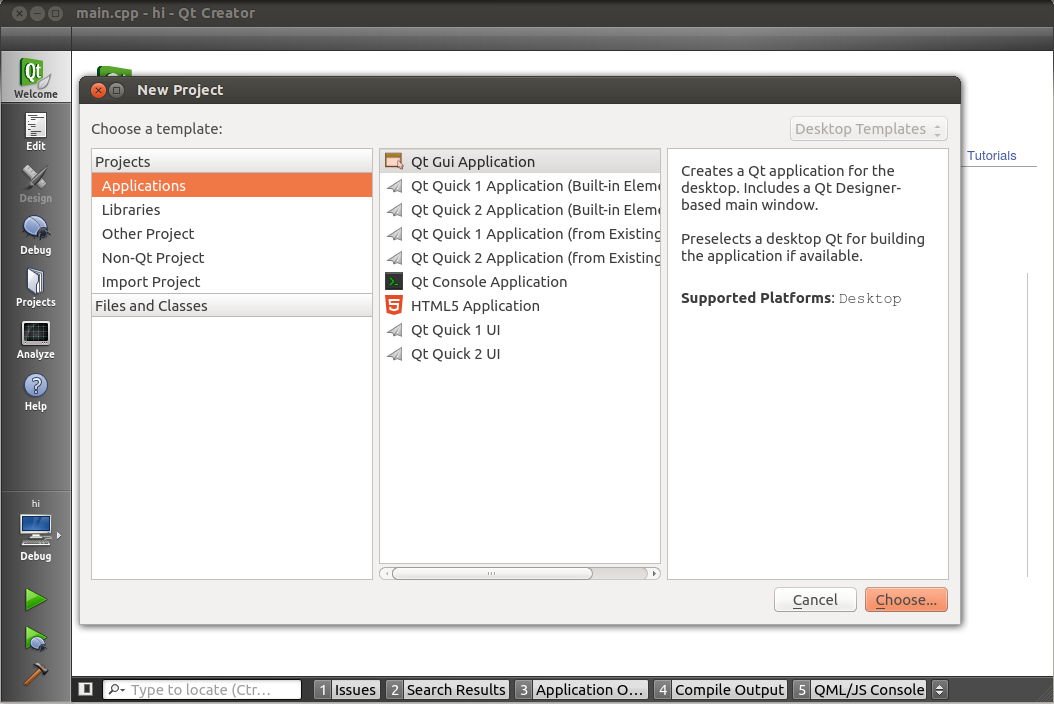
\includegraphics[scale=0.4]{images/new.png}
\caption{New file or project in Qt}
\end{center}
\end{figure}
In the  first  step,  the  user  selects  the  type of project from the categories. When  creating Qt Quick Projects,
the user can select either Qt Quick UI or Qt Quick Application.
A  Qt  Quick  UI  project  contains  a  single  QML  file  that  defines  the  main  view  of  the  application.  UI
designers  can  use  it  to  create  an  application  user  interface  and  review  it  in  the  QML  Viewer,  without
having  to  build  the  application.   UI  designers  do  not  need to have the development environment installed
on their computers to create and run this type of projects.
Developers  can  build  Qt  Quick  applications  and  deploy  them  on  mobile  target platforms. For example,
they  can  create  signed  Symbian  Installation  System  (SIS)  packages or Debian packages for this type of
project.  Developers  can  use  ready­made  Qt  Quick  Components  for  Symbian  and  MeeGo  Harmattan
that  allow  them  to  create  applications  with  a  native  look  and  feel  for  the  selected  mobile  platform.  The
components  are  delivered  as  part  of  Qt SDK. A Qt Quick UI project can be easily  converted into a Qt
Quick  application  by using the Qt Quick  application wizard to import the main QML file in the Qt Quick
UI project. The wizard prompts developers to enter the settings needed for a particular type of project.

\begin{figure}[h]
\begin{center}
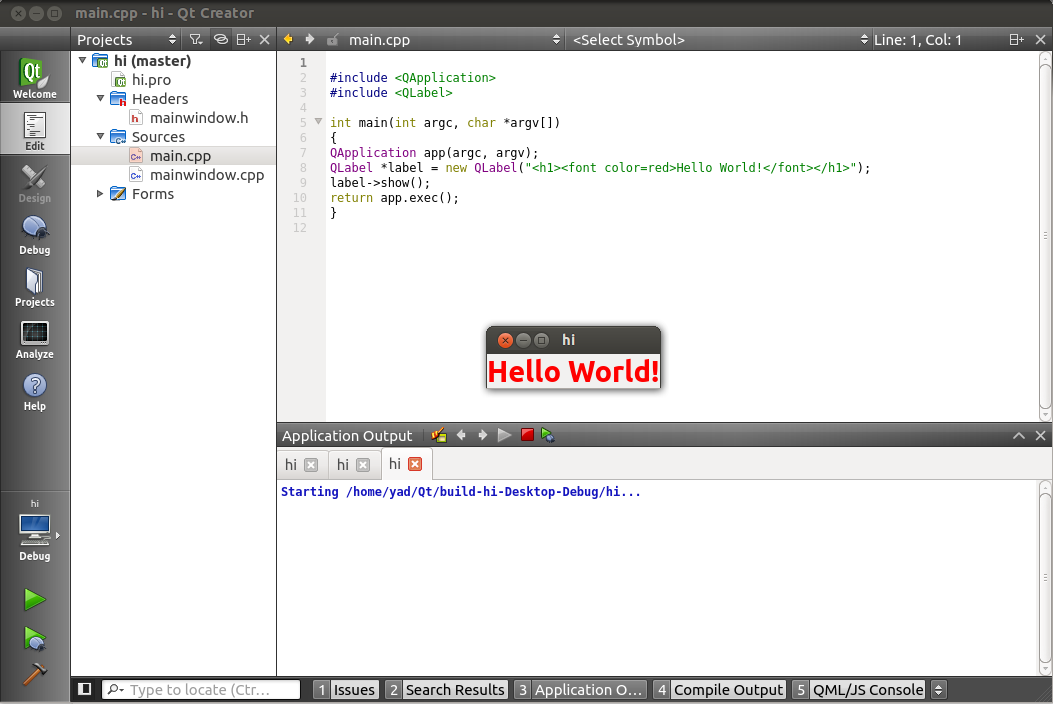
\includegraphics[scale=0.4]{images/hi.png}
\caption{Project to print hello word}
\end{center}
\end{figure}

When  the  steps  have  been  completed,  Qt  Creator  automatically  generates  the  project  with  required
headers,  source  files,  user  interface  descriptions  and  project  files,  as  defined  by  the  wizard.  Not  only
does  the  wizard  help  new  users  get  up  and  running  quickly,  it  also  enables  more  experienced  users  to
streamline  their  workflow  for  the  creation  of new projects. The convenient user interface makes it easier
to  ensure  that  a  project  begins  with  the  correct  configuration  and  dependencies.  Specifically,  the  Qt
Quick  application  wizard  allows  developers  to  create  projects  that  they  can  deploy  on  mobile  devices
with a click of the run button.
\\


\subsection{Using Qt Quick Toolbars}


When  users  edit  QML  code  in  the  code  editor,  they  specify  the  properties  of  QML   components.  For
some  properties,  such  as  colors   and  font  names,  this  is  not  a  trivial  task.  For  example,  few  people  can
visualize the color.
To  easily  edit these properties, users can employ the Qt Quick Toolbars. When a component is selected
in  the  code  and  a  toolbar  is  available,  a  light  bulb  icon  appears.  Users  select  the  icon  to  open  the
toolbar.
Qt  Quick  Toolbar  indicator  and  Qt  Quick  Toolbar  for  rectangles.  It  is  used  for  inserting  text,  images,
and  animation.  Qt  Quick  Toolbars  are  available  for  editing  the  properties  of  the  following  QML
elements:
● Rectangles
● Text
● Images
● Animation


\subsection{Deploying Applications to Mobile Devices}

Qt Creator deploy configurations handle the packaging of the application as an executable and copying it
to  a  location  developers  want  to  run  the  executable  at.  The  files  can  be  copied  to  a  location  in  the  file
system  of  the  development  PC  or  a  mobile  device.  To  deploy  files  on  mobile devices, developers must
either  connect  the  devices  to  the  development  PC  or  use  the  installation  packages  generated  by  Qt
Creator.  Qt  Quick  UI  projects  must  be  converted into Qt Quick applications for deployment on mobile devices.
Qt  Creator  allows developers to  create installation packages for Symbian, MeeGo, and Maemo devices
that are suitable for publishing on Ovi Store.


%----------------------------------------------------------------------------------------
\
\
\
%-------------------------------------------------------------------


\subsection{Getting Help}

From  time  to  time,  developers  may  need  further  information  about  a  certain  QML  element,  Qt  class,
function,  or  other  part  of  the  Qt  API.  All   the  Qt  documentation  and  examples are accessible via the Qt
Help plugin in Qt Creator.
To  view  the  documentation,   the  Help  mode  is  used,  where  most  of  the  window  is  devoted  to  the  help
text.  While working with source code in Edit mode, the user can access context sensitive help by moving
the  text  cursor  to  a  Qt  class  or   function  and  then  press  the  F1  key.  The  documentation  is  displayed
within a panel on the right side of the code editor, as shown in the following figure.

Qt  Designer  is  a  powerful cross­platform GUI layout and forms builder. It allows you to rapidly design
and  build  widgets  and  dialogs  using  on­screen  forms  using  the  same  widgets  that  will  be  used  in  your
application.  Forms  created  with  Qt  Designer  are fully­functional, and they can be previewed so that you
can ensure that they will look and feel exactly as you intended.\\


%----------------------------------------------------------------------------------------

%-------------------------------------------------------------------

\begin{small}
\subsection{\large Features and Benefits}
\end{small}
\begin{itemize}
\item Design user interfaces quickly with drag and drop functionality
\item Customize widgets or choose from library of standard widgets
\item Instantly preview forms in native look and feel
\item Generate C++ or Java code from your interface prototypes
\item Use Qt Designer with Visual Studio or Eclipse IDEs
\item Build fully­functional user interfaces with Qt’s signals and slots
\end{itemize}
\begin{figure}[htb]
\begin{center}
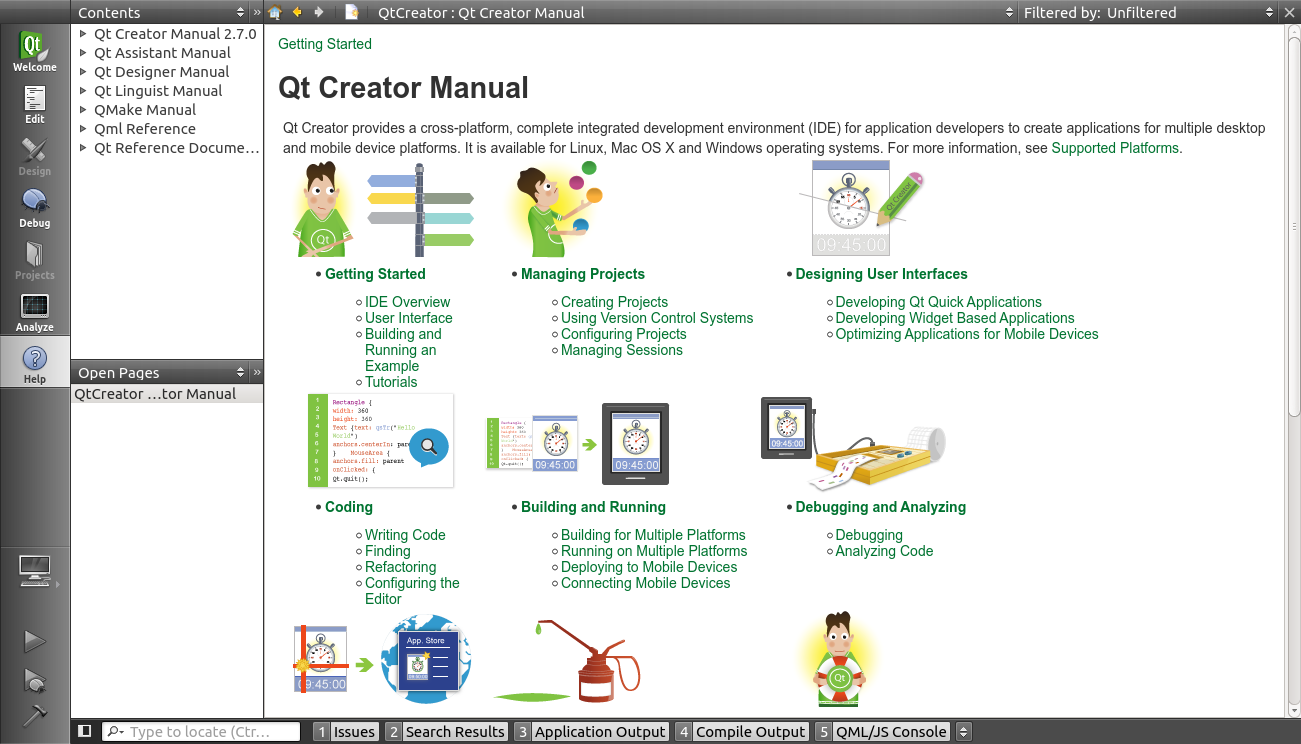
\includegraphics[scale=0.4]{images/Qtman.png}
\caption{ Displaying context sensitive Qt Help information}
\end{center}
\end{figure}